%Introductory sentences here

Critically, the learned generative model is used to generate the data for training the evaluative model. To achieve this the generative model is presented with a simulated depth image of a scene containing a single unfamiliar object. Using this, grasps are generated and executed in simulation. The success or failure of each simulated grasp is recorded. Producing a good simulation for evaluating grasps is a non-trivial matter, and so we describe the choices we made below. A particularly important problem in our case is that the resulting data set must capture the uncertainty in unobservable variables, such as mass and friction. Our approach leads to what we term {\em robust evaluation}.

\subsection{Features and Constraints of the Virtual Environment}
\label{subsection:environment}
In summary, the main features of our grasp simulation are as follows.
\begin{itemize}
\item MuJoCo \cite{MuJoCo} has been chosen as the base physics simulator. 
\item 3D models of 294 objects drawn from 20 categories are employed.
\item To support dynamics simulation, each 3D model is decomposed into convex parts using V-HACD method \cite{V-HACD}.
\item Prior distributions for mass, size and frictional coefficient were estimated using real-world data. The properties of simulated objects are sampled from these priors.
\item MuJoCo is configured to use an impedance controller to control the DLR-II hand in simulation.
\item In order to simulate the Carmine 1.09 depth sensor installed on the robot, a modified version of the Blensor Kinect sensor simulator \cite{KinectSimulator} has been used. 
\item For each object, we varying the camera orientation and distance from the object, as well as object mass, friction, scale, location and orientation. 
\item A 3D mesh-model of the DLR-II hand has been used in the simulator. There are no kinematic constraints on how the hand can grasp an object, other than collisions with the virtual table where the objects reside. 
\end{itemize}

The reasons for the most critical of these decisions are now given in slightly more detail. First, in order to create a realistic simulation environment, we chose the MuJoCo \cite{MuJoCo} physics simulator over other simulators (OpenSim, BulletPhysics, ODE, NVIDIA PhysX) for two reasons: 
\begin{itemize}
\item MuJoCo uses generalized coordinates and optimization-based contact dynamics, resulting in fewer numerical instabilities,
\item MuJoCo is optimized for the quality of physics as well as its speed, hence improving the quality of the physics simulation.
\end{itemize}

Due to the fact that MuJoCo needs objects to consist of convex parts for collision checks, all 294 objects in the model dataset was decomposed into convex parts. Figure~\ref{fig:objectDecomposition} approximates decompositions of some objects in our dataset, using the V-HACD algorithm \cite{V-HACD}. The number of sub-parts for all objects in our dataset varies between 2-120. 
\begin{figure}
  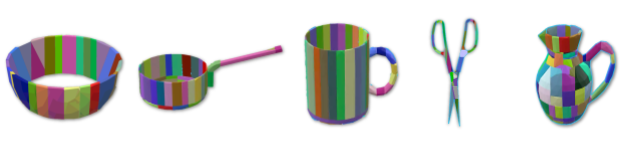
\includegraphics[width=\linewidth]{images/decomposition.png}
  \caption{Approximate convex decomposition of some objects in our dataset. Best viewed in colour.}
  \label{fig:objectDecomposition}
\end{figure}
The dataset of 294 objects is drawn from 20 classes and includes: bottles, bowls, cans, boxes, kitchen utensils, mugs, cups, pans and other graspable objects such as tennis balls and dust pans, as seen in Figure \ref{fig:allObjects}. All objects used in the simulation are chosen to have a size that is within the grasp aperture limit of the DLR-II hand. The number of objects in each class varies from 1 (dustpan) to 25 (bottles). 250 objects from all classes were used for training the network, while the remaining 44 were used for testing. The objects are everyday objects. Examples are kitchen objects such as bowls, plates, mugs and teacups, solid objects such as boxes and balls, kitchen utensils such as spatulas, spoons. Long/thin objects such as spatulas, forks, spoons, and knives are placed vertically in a short, heavy stand in order to make them graspable without touching the table. 

\subsection{Data Collection Methodology}
\label{subsection:dataCollection}

In order to fully learn the relationship between visual cues, grasp parameters and grasp success, we  consider the hand as having a free joint where the only constraint on its movement is collisions with the table. We divided the data collection process into units called \textit{scenes}, where each scene has a single object placed on a table, and then a number of grasps are attempted in that scene, so as to pick up the object. Below, we specify the time flow of data collection:

\begin{enumerate}
\item A novel instance of an object from the dataset is generated and placed on a virtual table. Variations applied include object position, orientation, scale, weight and friction coefficients. This variation is critical to ensuring that the evaluative model will predict the robustness of a grasp to variations in the conditions.
\item A simulated depth camera takes a depth image $I_s$ of the scene, converting it into a point cloud $P_s$. The ${elevation}_s$ of the camera view point varies between 30-57 degrees, whereas the ${azimuth}_s$ is sampled from $[0, 2\pi]$. 
\item The grasp generator algorithm by \citet{kopicki2015ijrr} is used to generate a number of candidate grasps $H = \{h_i\}_{i=0}^{K}$. The top 10 grasps from all 10 grasp types are picked and applied to the object in simulation.
\item More simulated depth images are taken from other virtual cameras around the object. The locations and orientations of these cameras are determined based on the same distribution where the initial image was taken, as explained in step 2. Up to 20 images are acquired, and a random view is associated with each grasp created in step 3. 
\item Results, including grasp success outcome, grasp information and depth image are stored for every trial. The grasp parameters are converted to the frame of reference of the associated view for every grasp.
\end{enumerate}

%Each candidate grasp $h_i = \{w_0, ..., w_{n}\}$ consists of a series of 10 waypoints along : $w_0$, ..., $w_{n}$. A waypoint $w_k$ is a 27-element vector that specifies full configuration of the hand in joint space: 3 dimensions for 3D coordinates and 4 dimensions for the orientation of the wrist, and 20 parameters specifying each finger joint's activation. 

After a grasp $h_i$ is generated in world coordinates, the waypoints that belong to the grasp are converted to the camera's frame of reference. The key goal of our network architecture is to learn which grasps are more likely to succeed given a point cloud, where both input channels are represented in terms of the camera frame of reference. %This point differentiates us from the work of Levine et al. \cite{Levine1}, where camera coordinates are not used. It should be noted that the possible camera locations in our simulated data covers a larger space, with full circular movement $[0, 2\pi]$ on azimuth and $[30-57]$ range in elevation. Our scenes do not have any distinguishing landmarks such as a bin or robot base, which may aid the network in locating the camera in the scene. 

In each scene $S_i$, a number of depth images are taken $\{I_{ik}\}_{k=0}^20$, in the manner explained above. The first image $I_{i0}$ is used to generate grasps, as explained in Section \ref{section:generative}. We use up to 20 distinct views in each scene, while we typically perform 100 grasps. Attaching different views to each grasp instead of using the seed image $I_{i0}$ ensures there is more variation in terms of viewpoints, resulting in a richer dataset. 20 has been chosen, as sampling one view per grasp would introduce a large overhead. Typically, performing a grasp takes half of the time it takes to acquire an image using the simulated camera.

Once a grasp is performed in simulation, it is considered a success if an object is lifted 1 meter above the table, and held there for another 2 seconds. If the object slips from the hand during lifting or holding, the grasp is a failure. 

\begin{figure}[t]
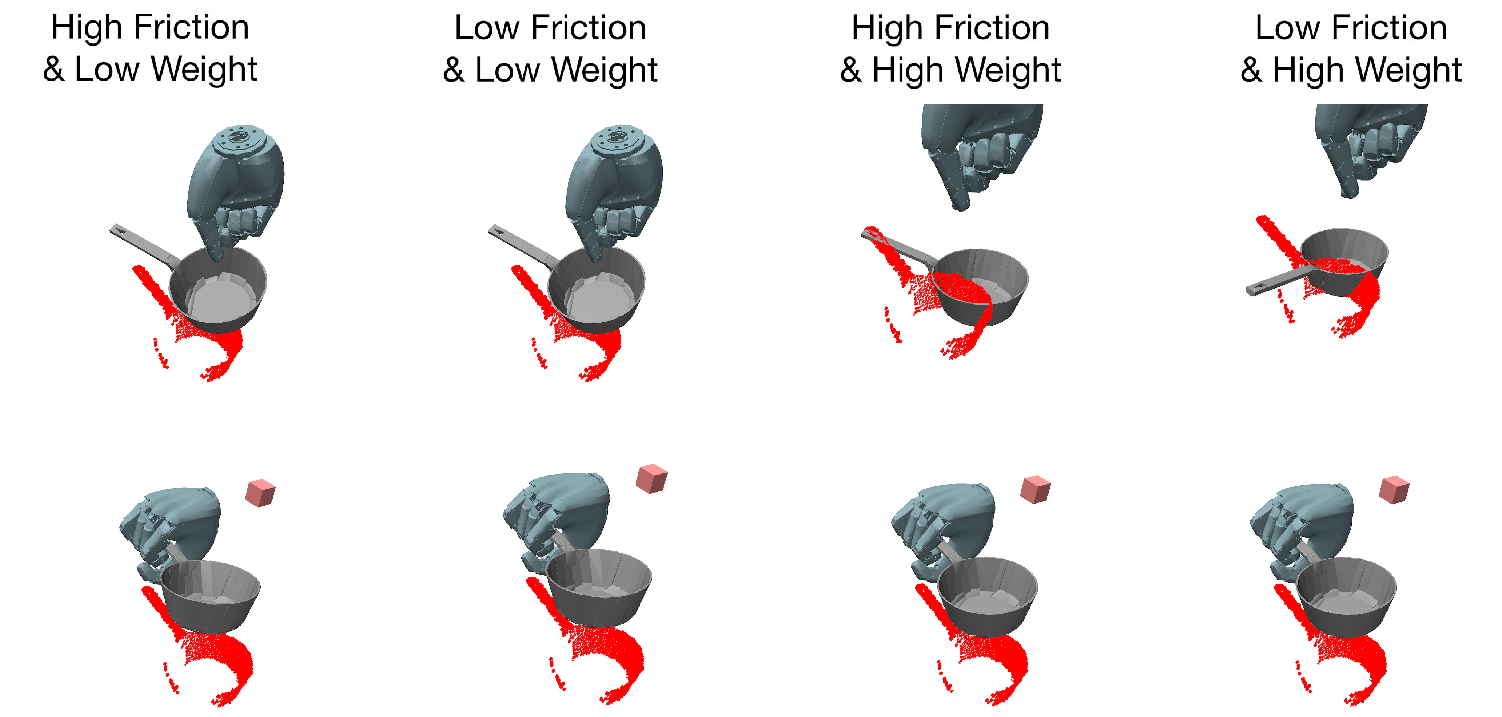
\includegraphics[width=\columnwidth]{images/frictionweight}
%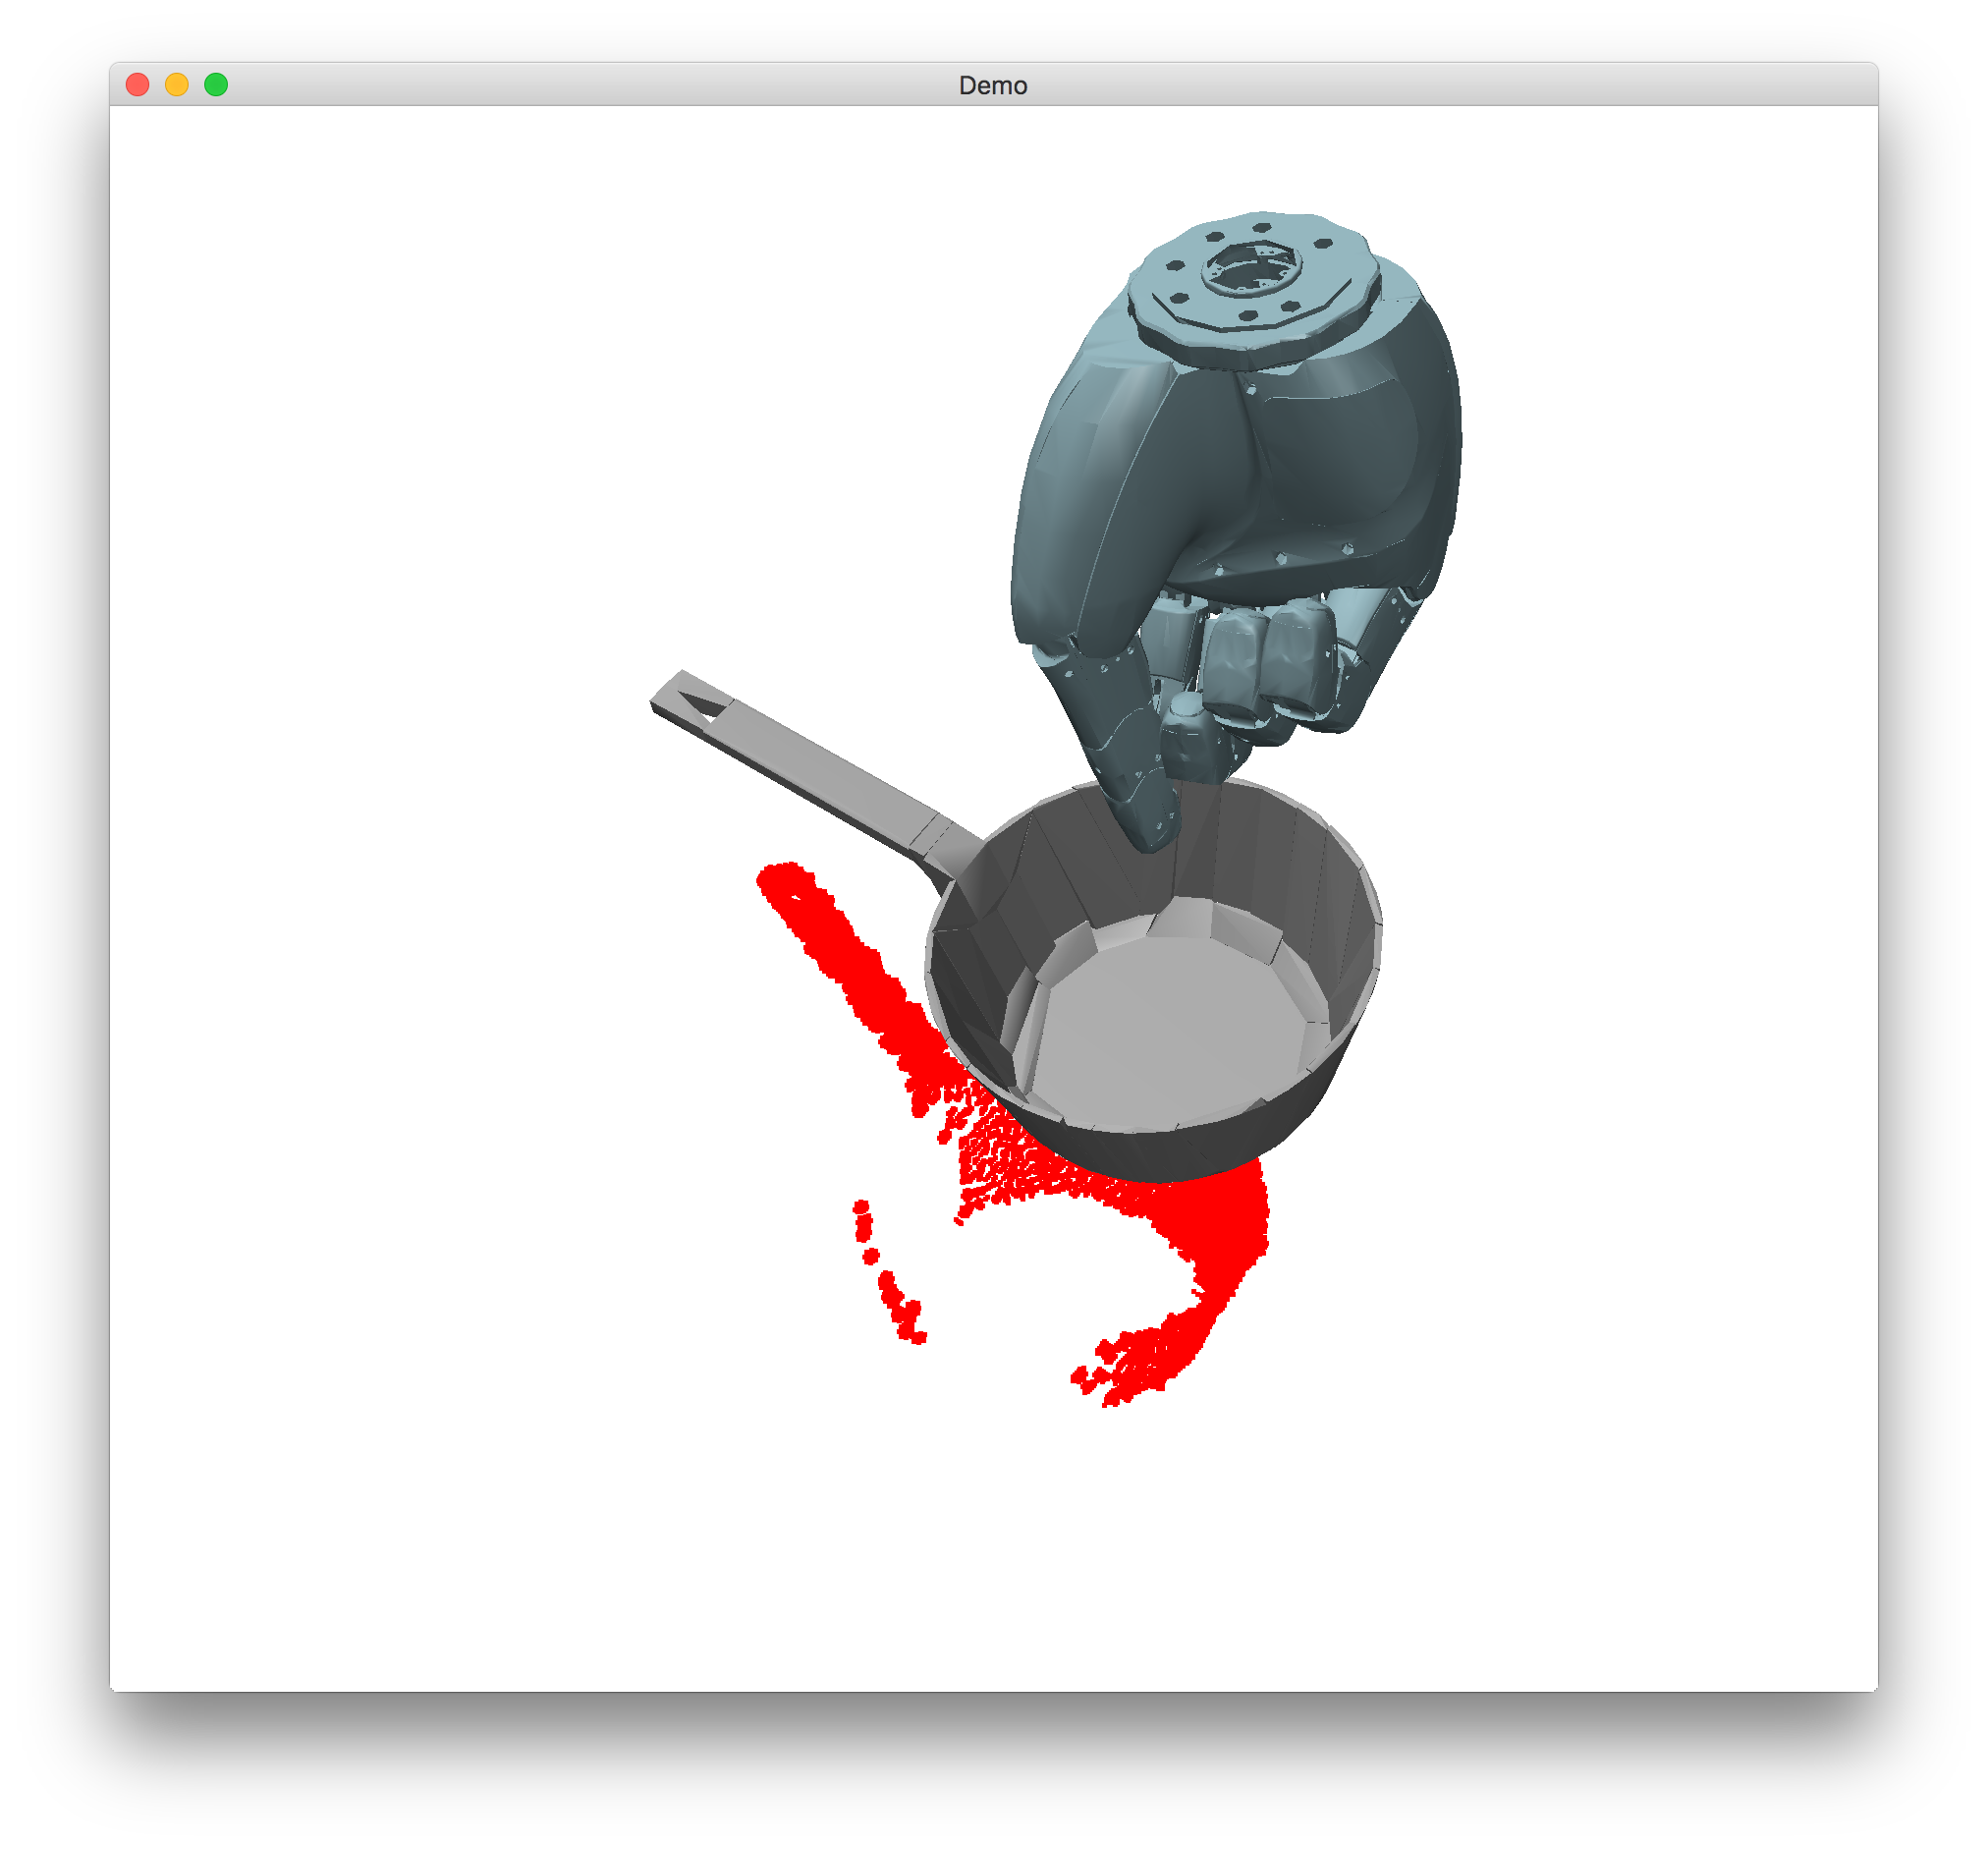
\includegraphics[width=0.24\textwidth]{images/Pan4_2_HFLW}
%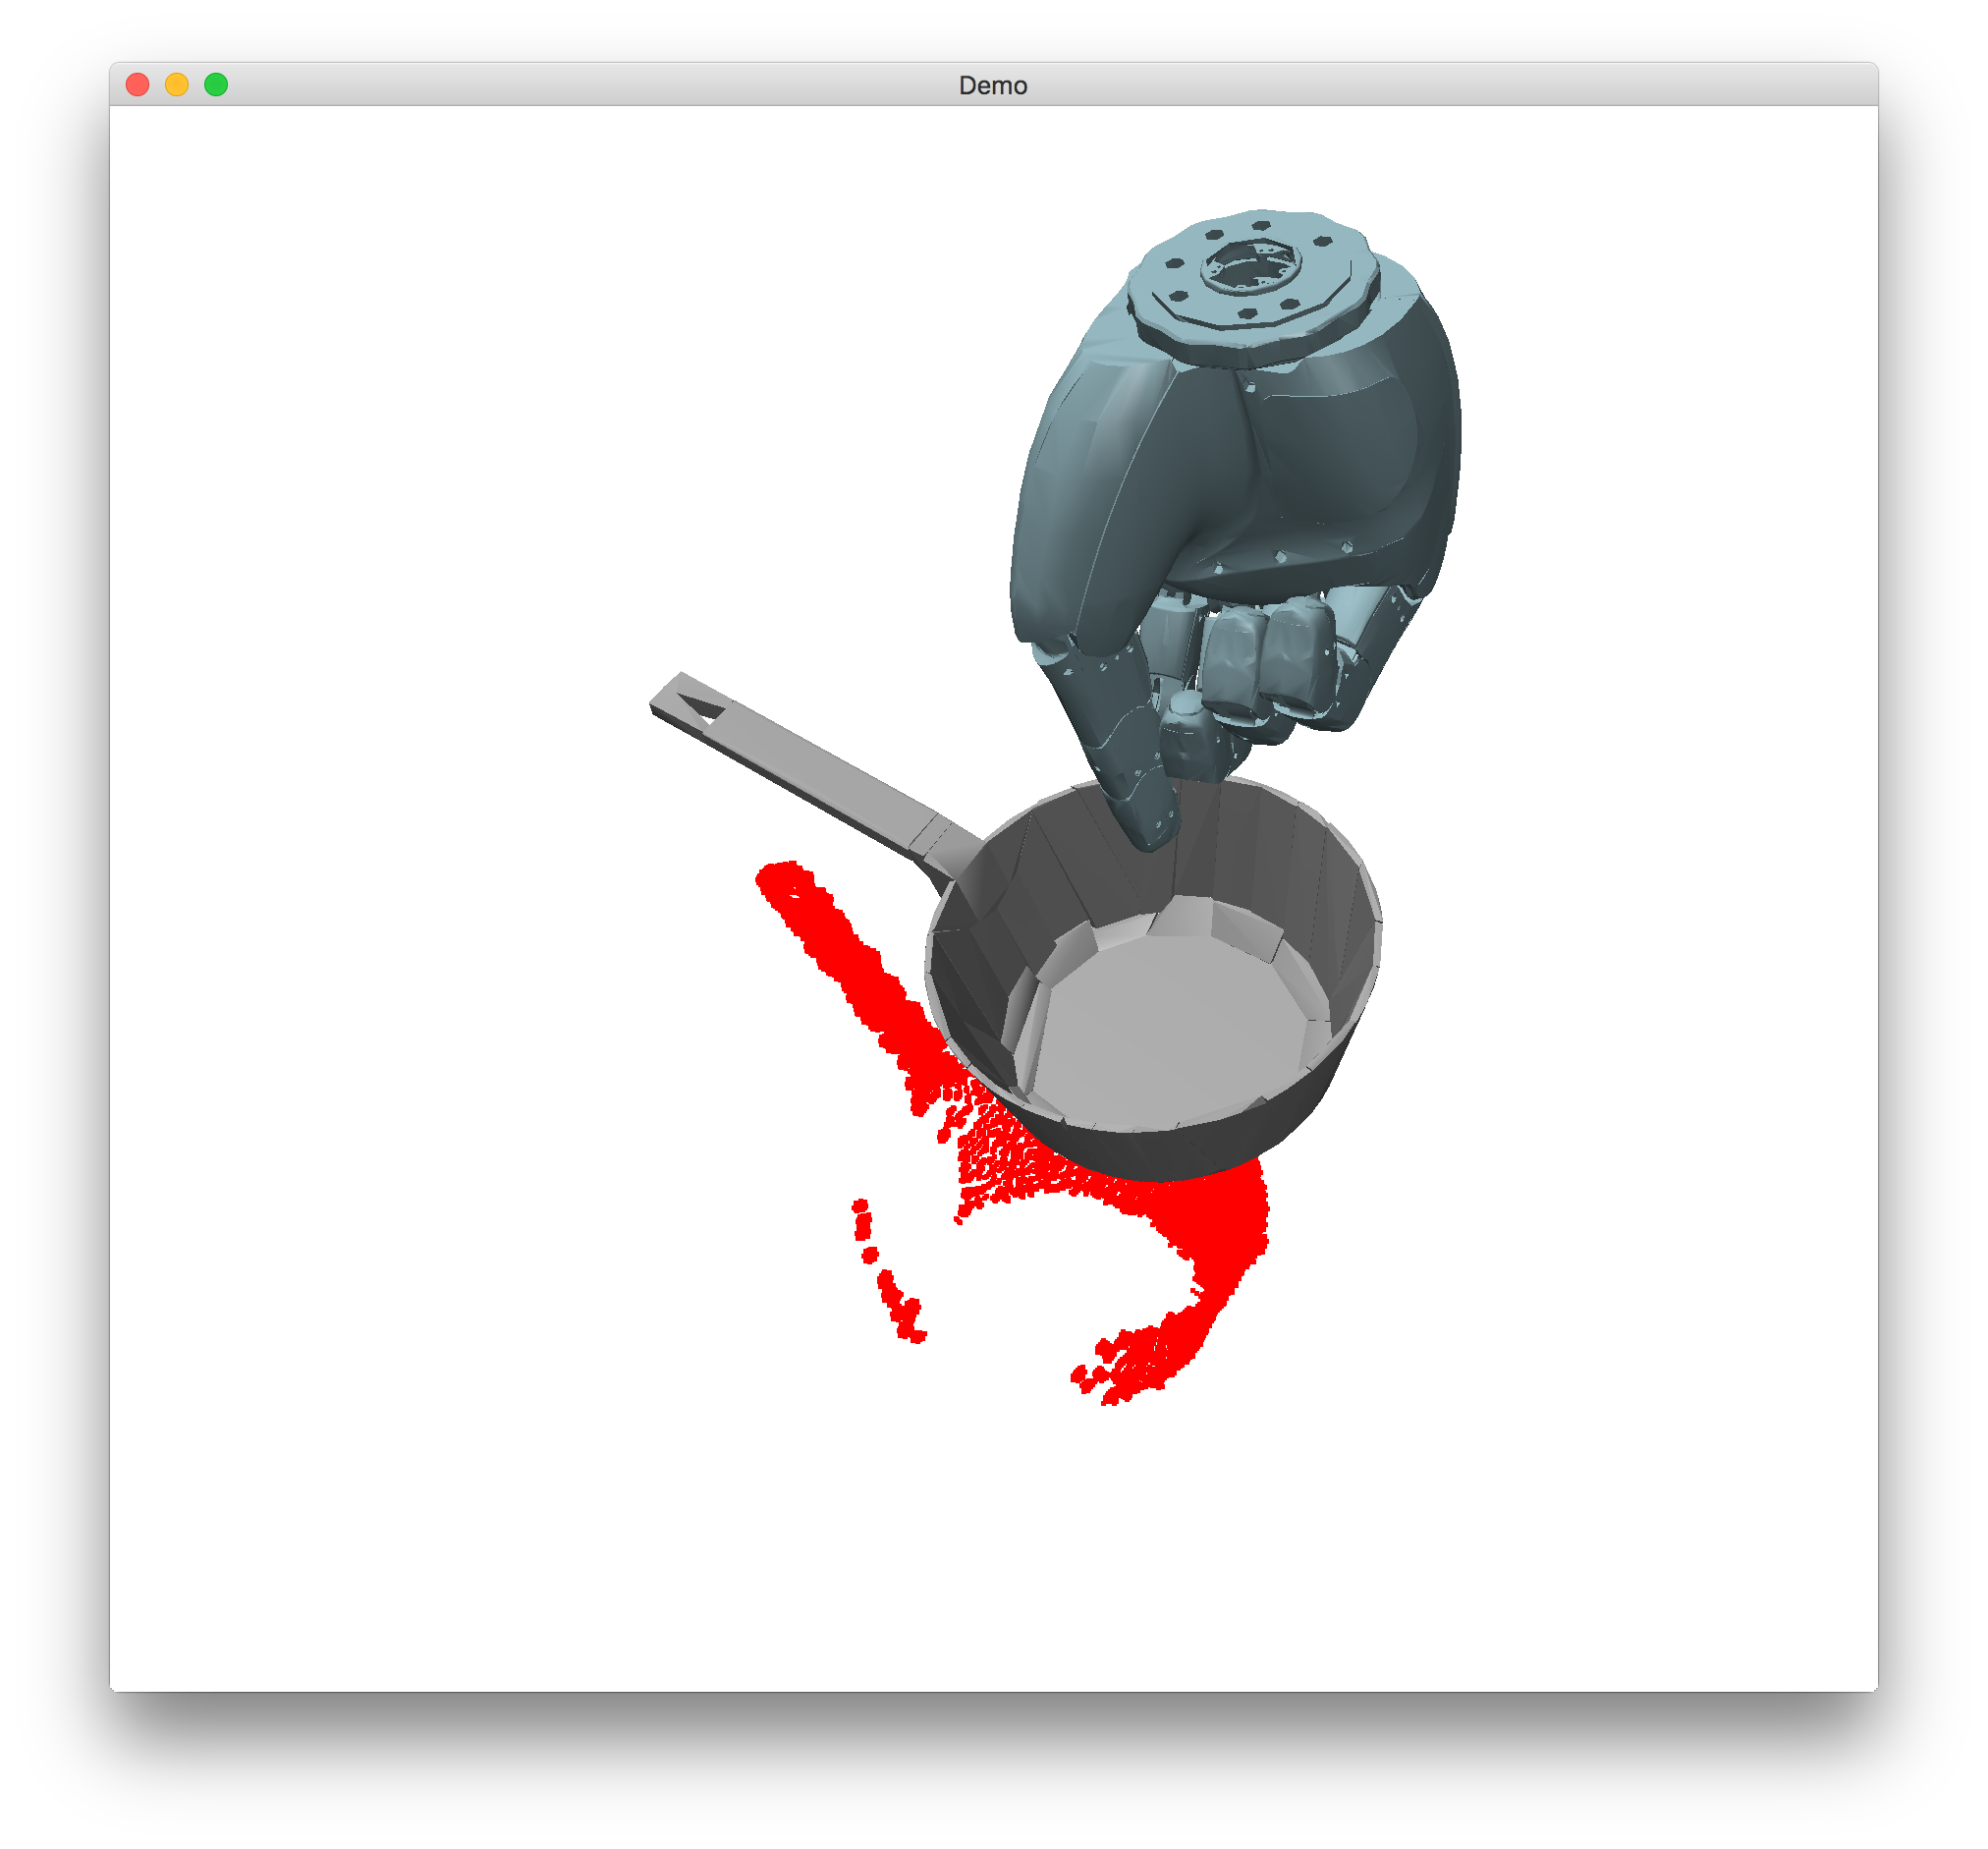
\includegraphics[width=0.24\textwidth]{images/Pan4_2_LFLW}
%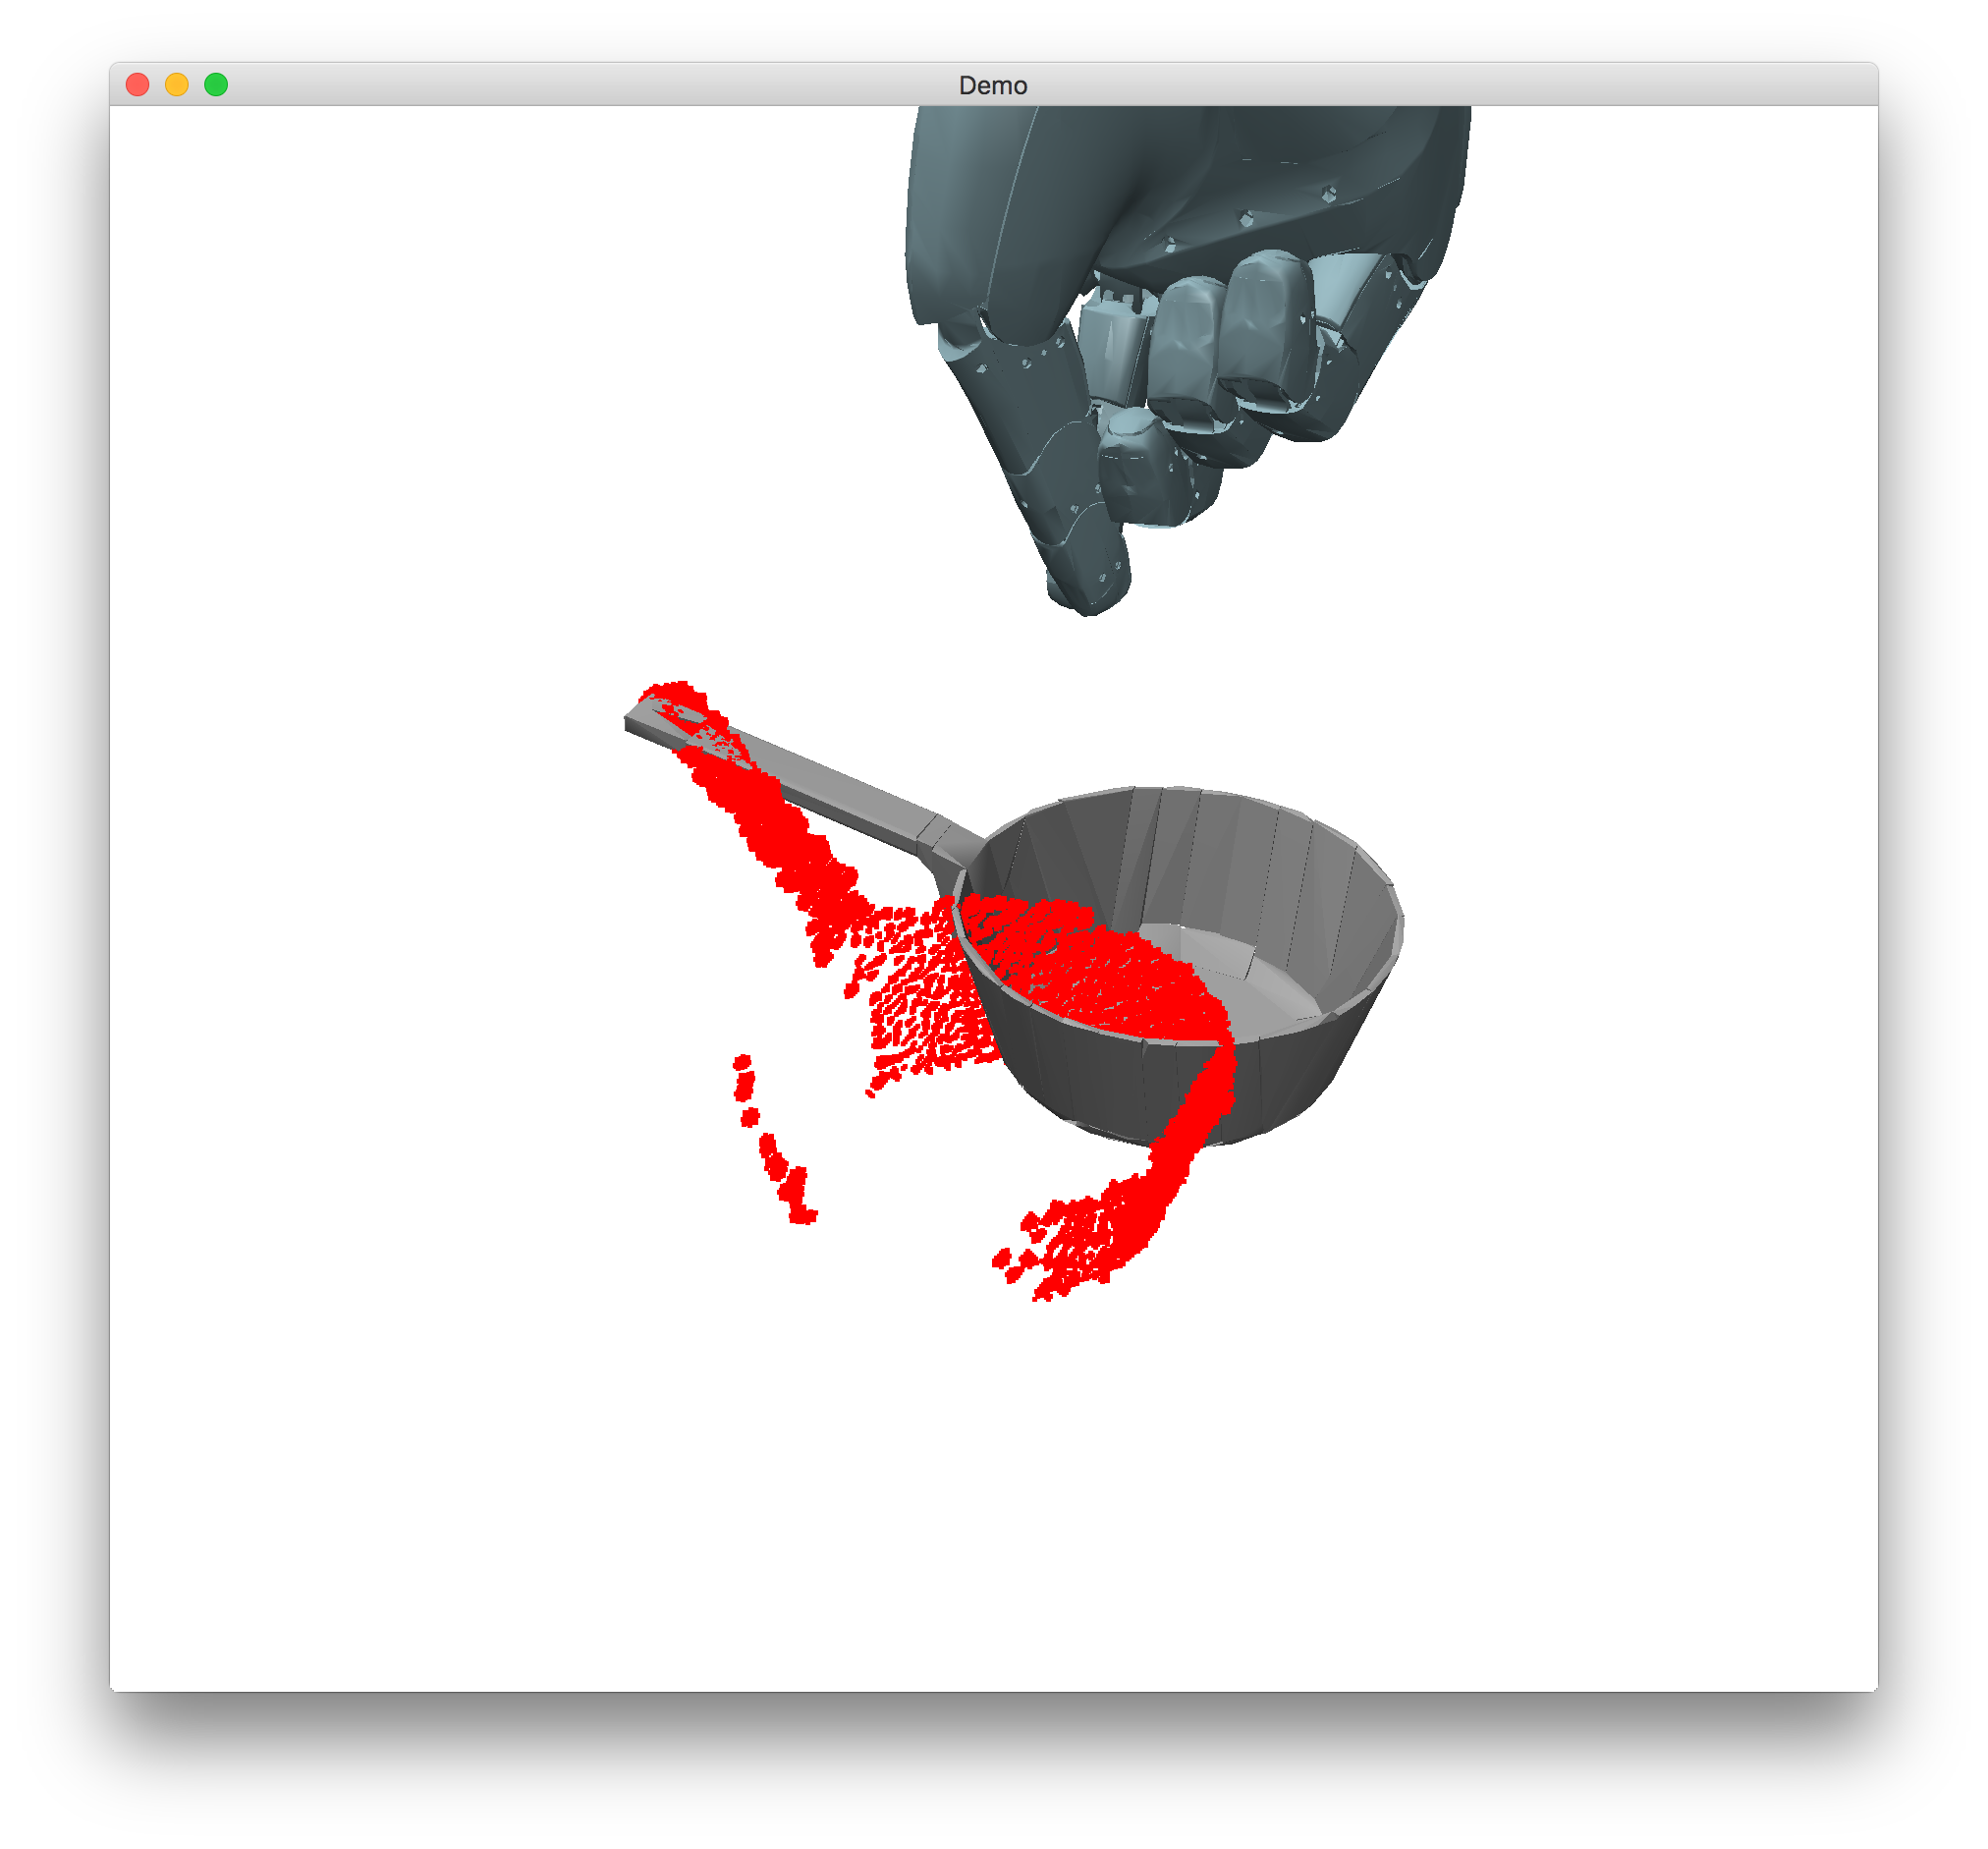
\includegraphics[width=0.24\textwidth]{images/Pan4_2_HFHW}
%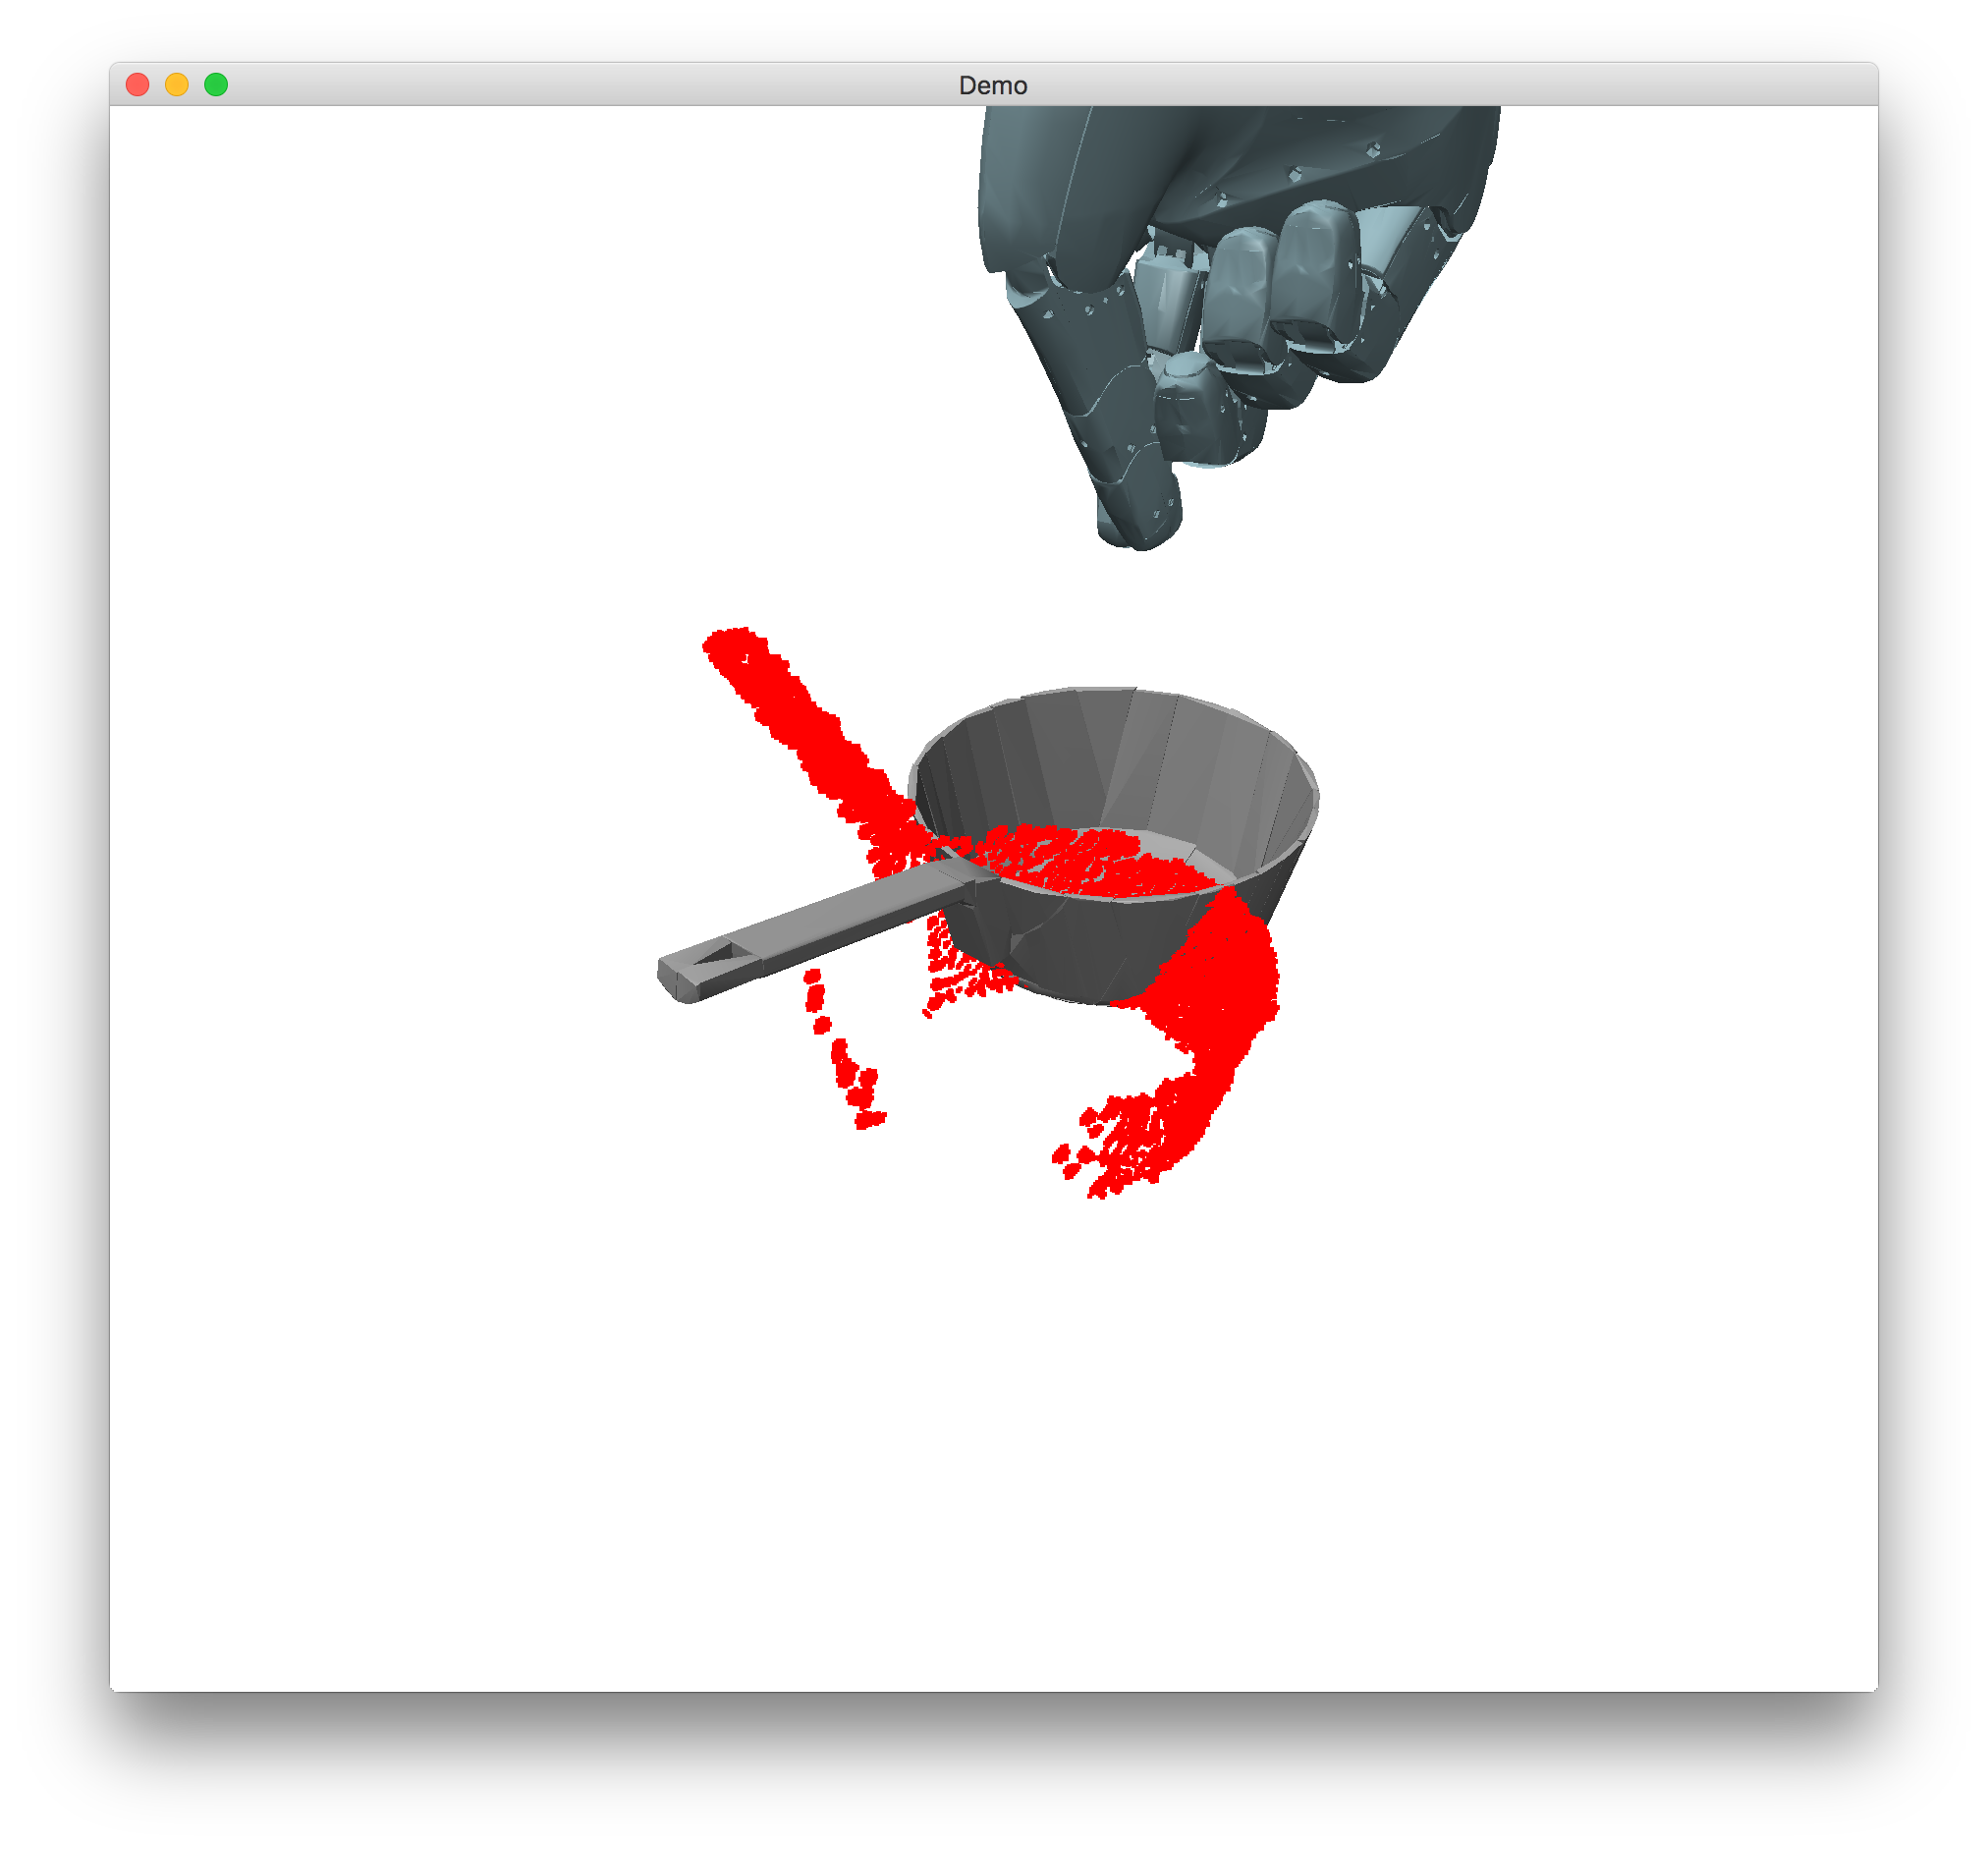
\includegraphics[width=0.24\textwidth]{images/Pan4_2_LFHW}\\
%%
\includegraphics[width=0.96\textwidth]{images/key-to-eval-training}\\
%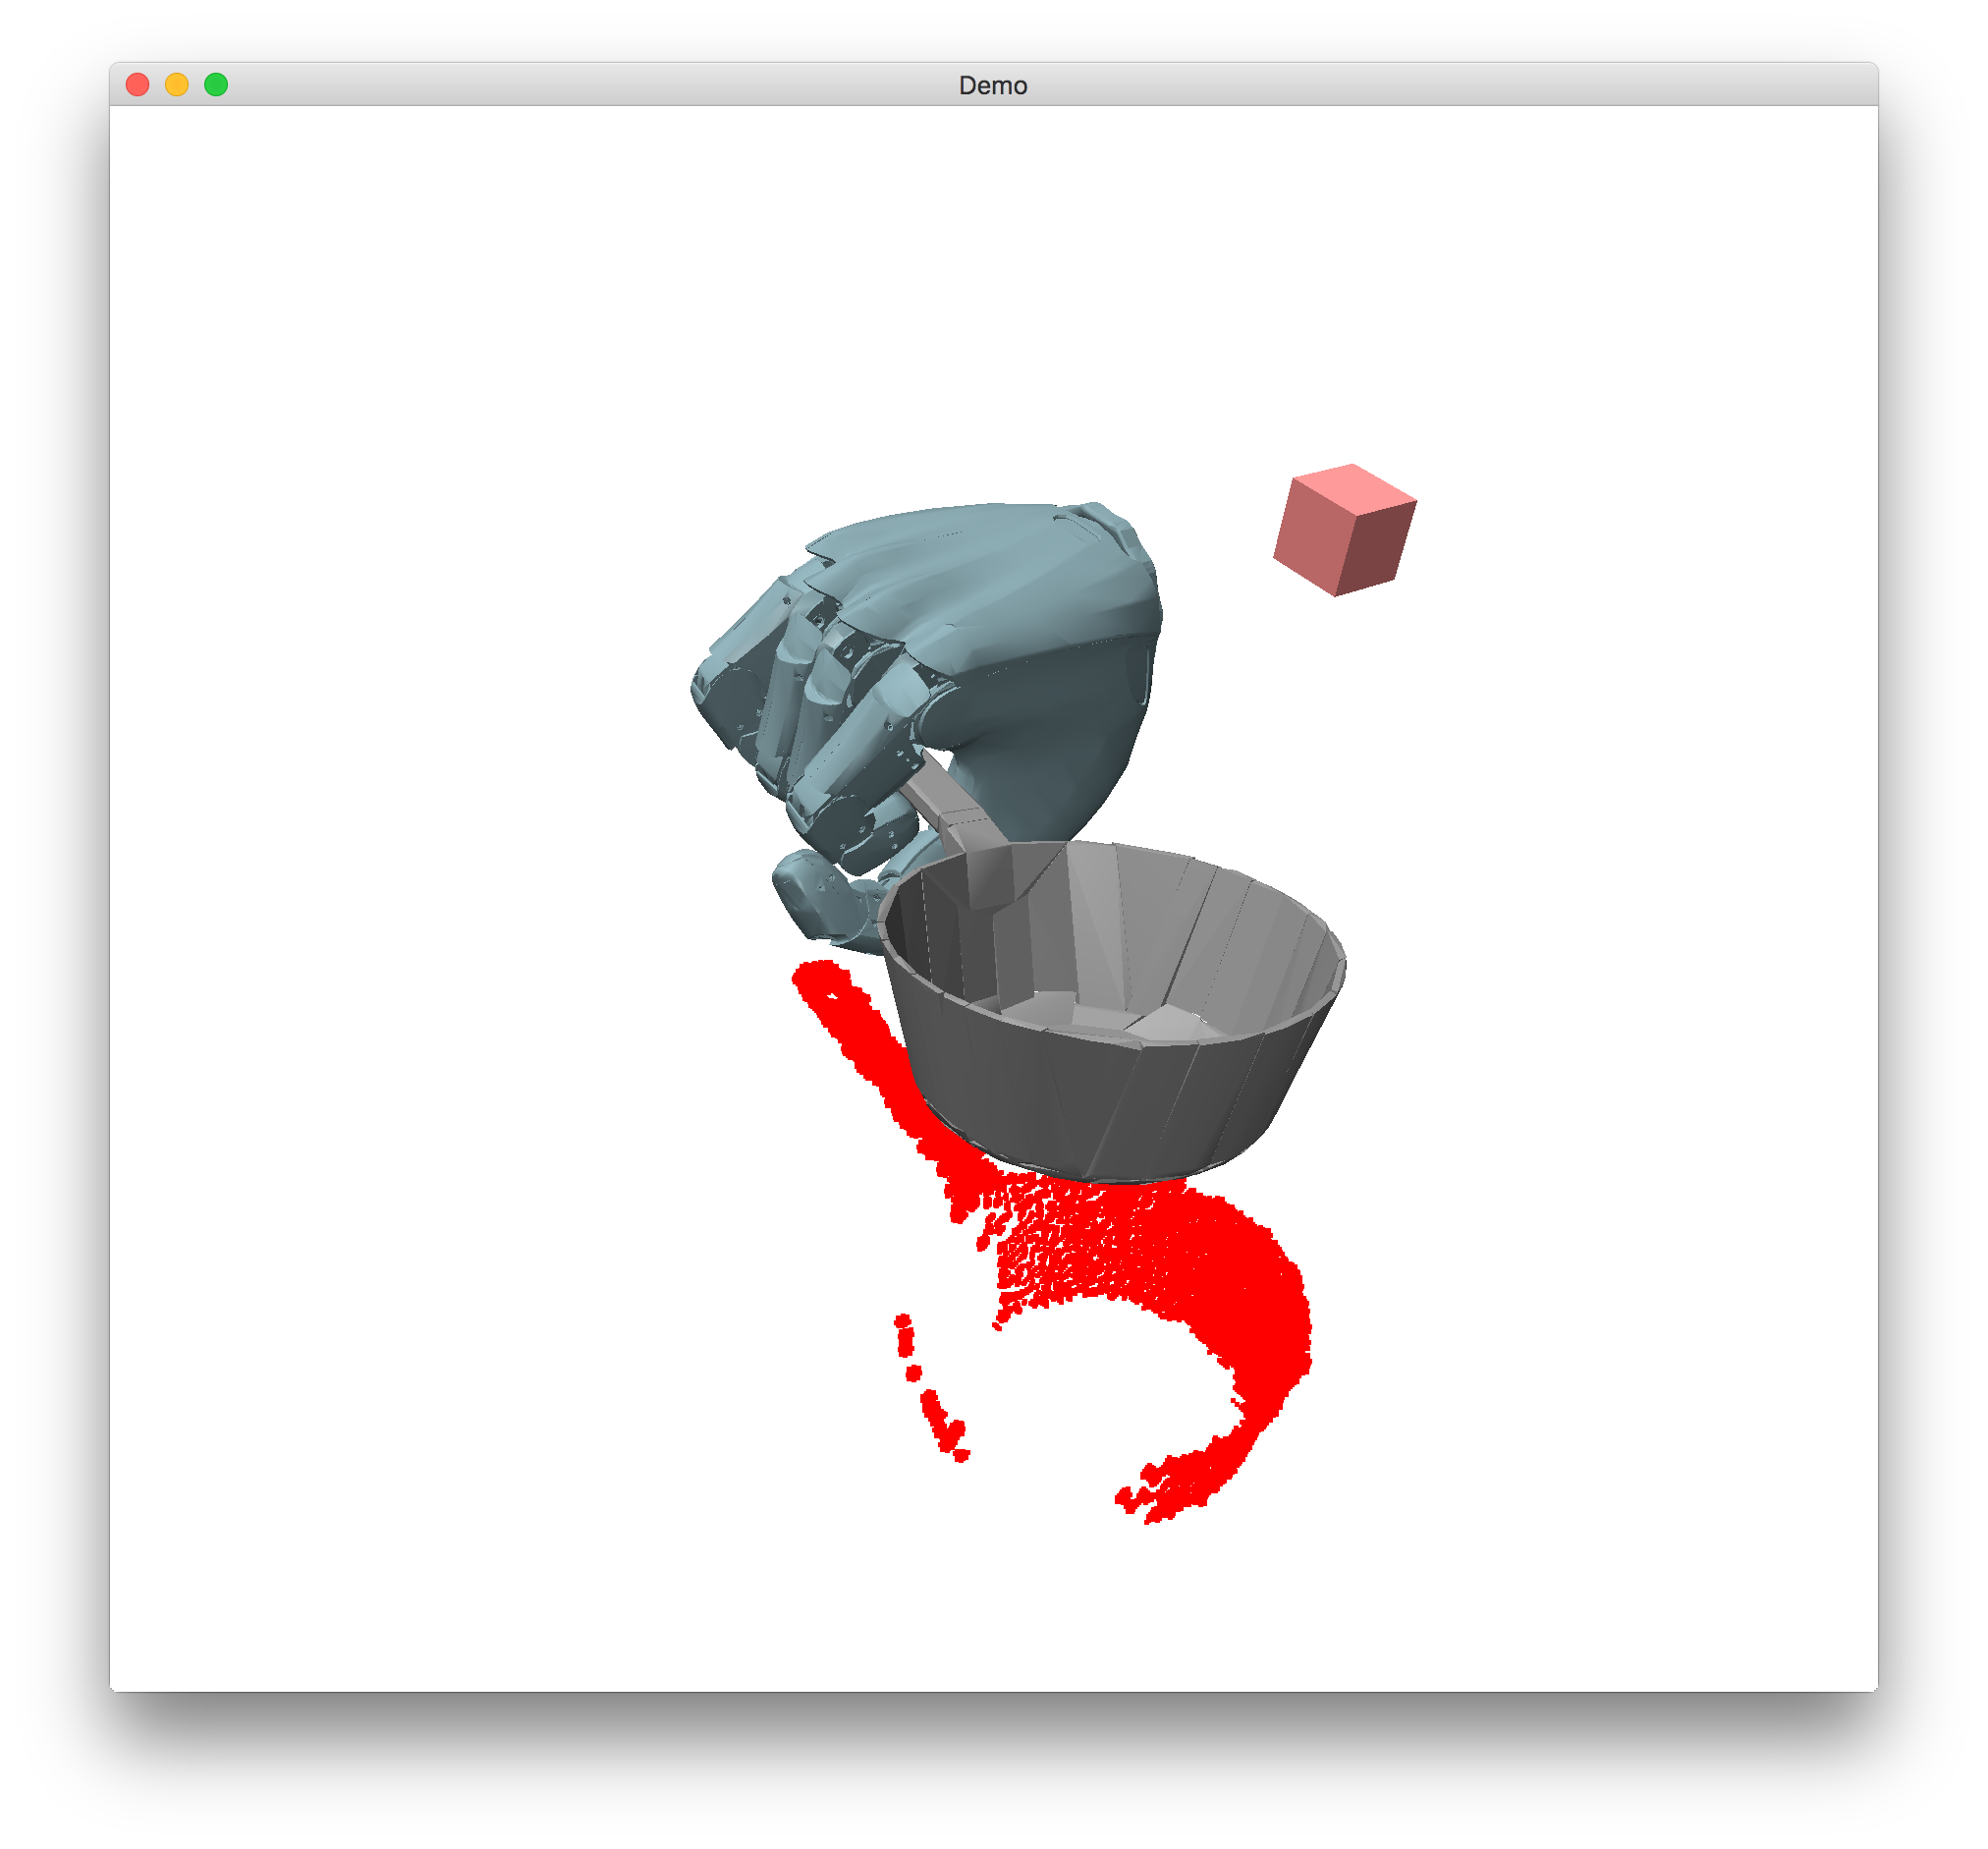
\includegraphics[width=0.24\textwidth]{images/Pan4_HFLW}
%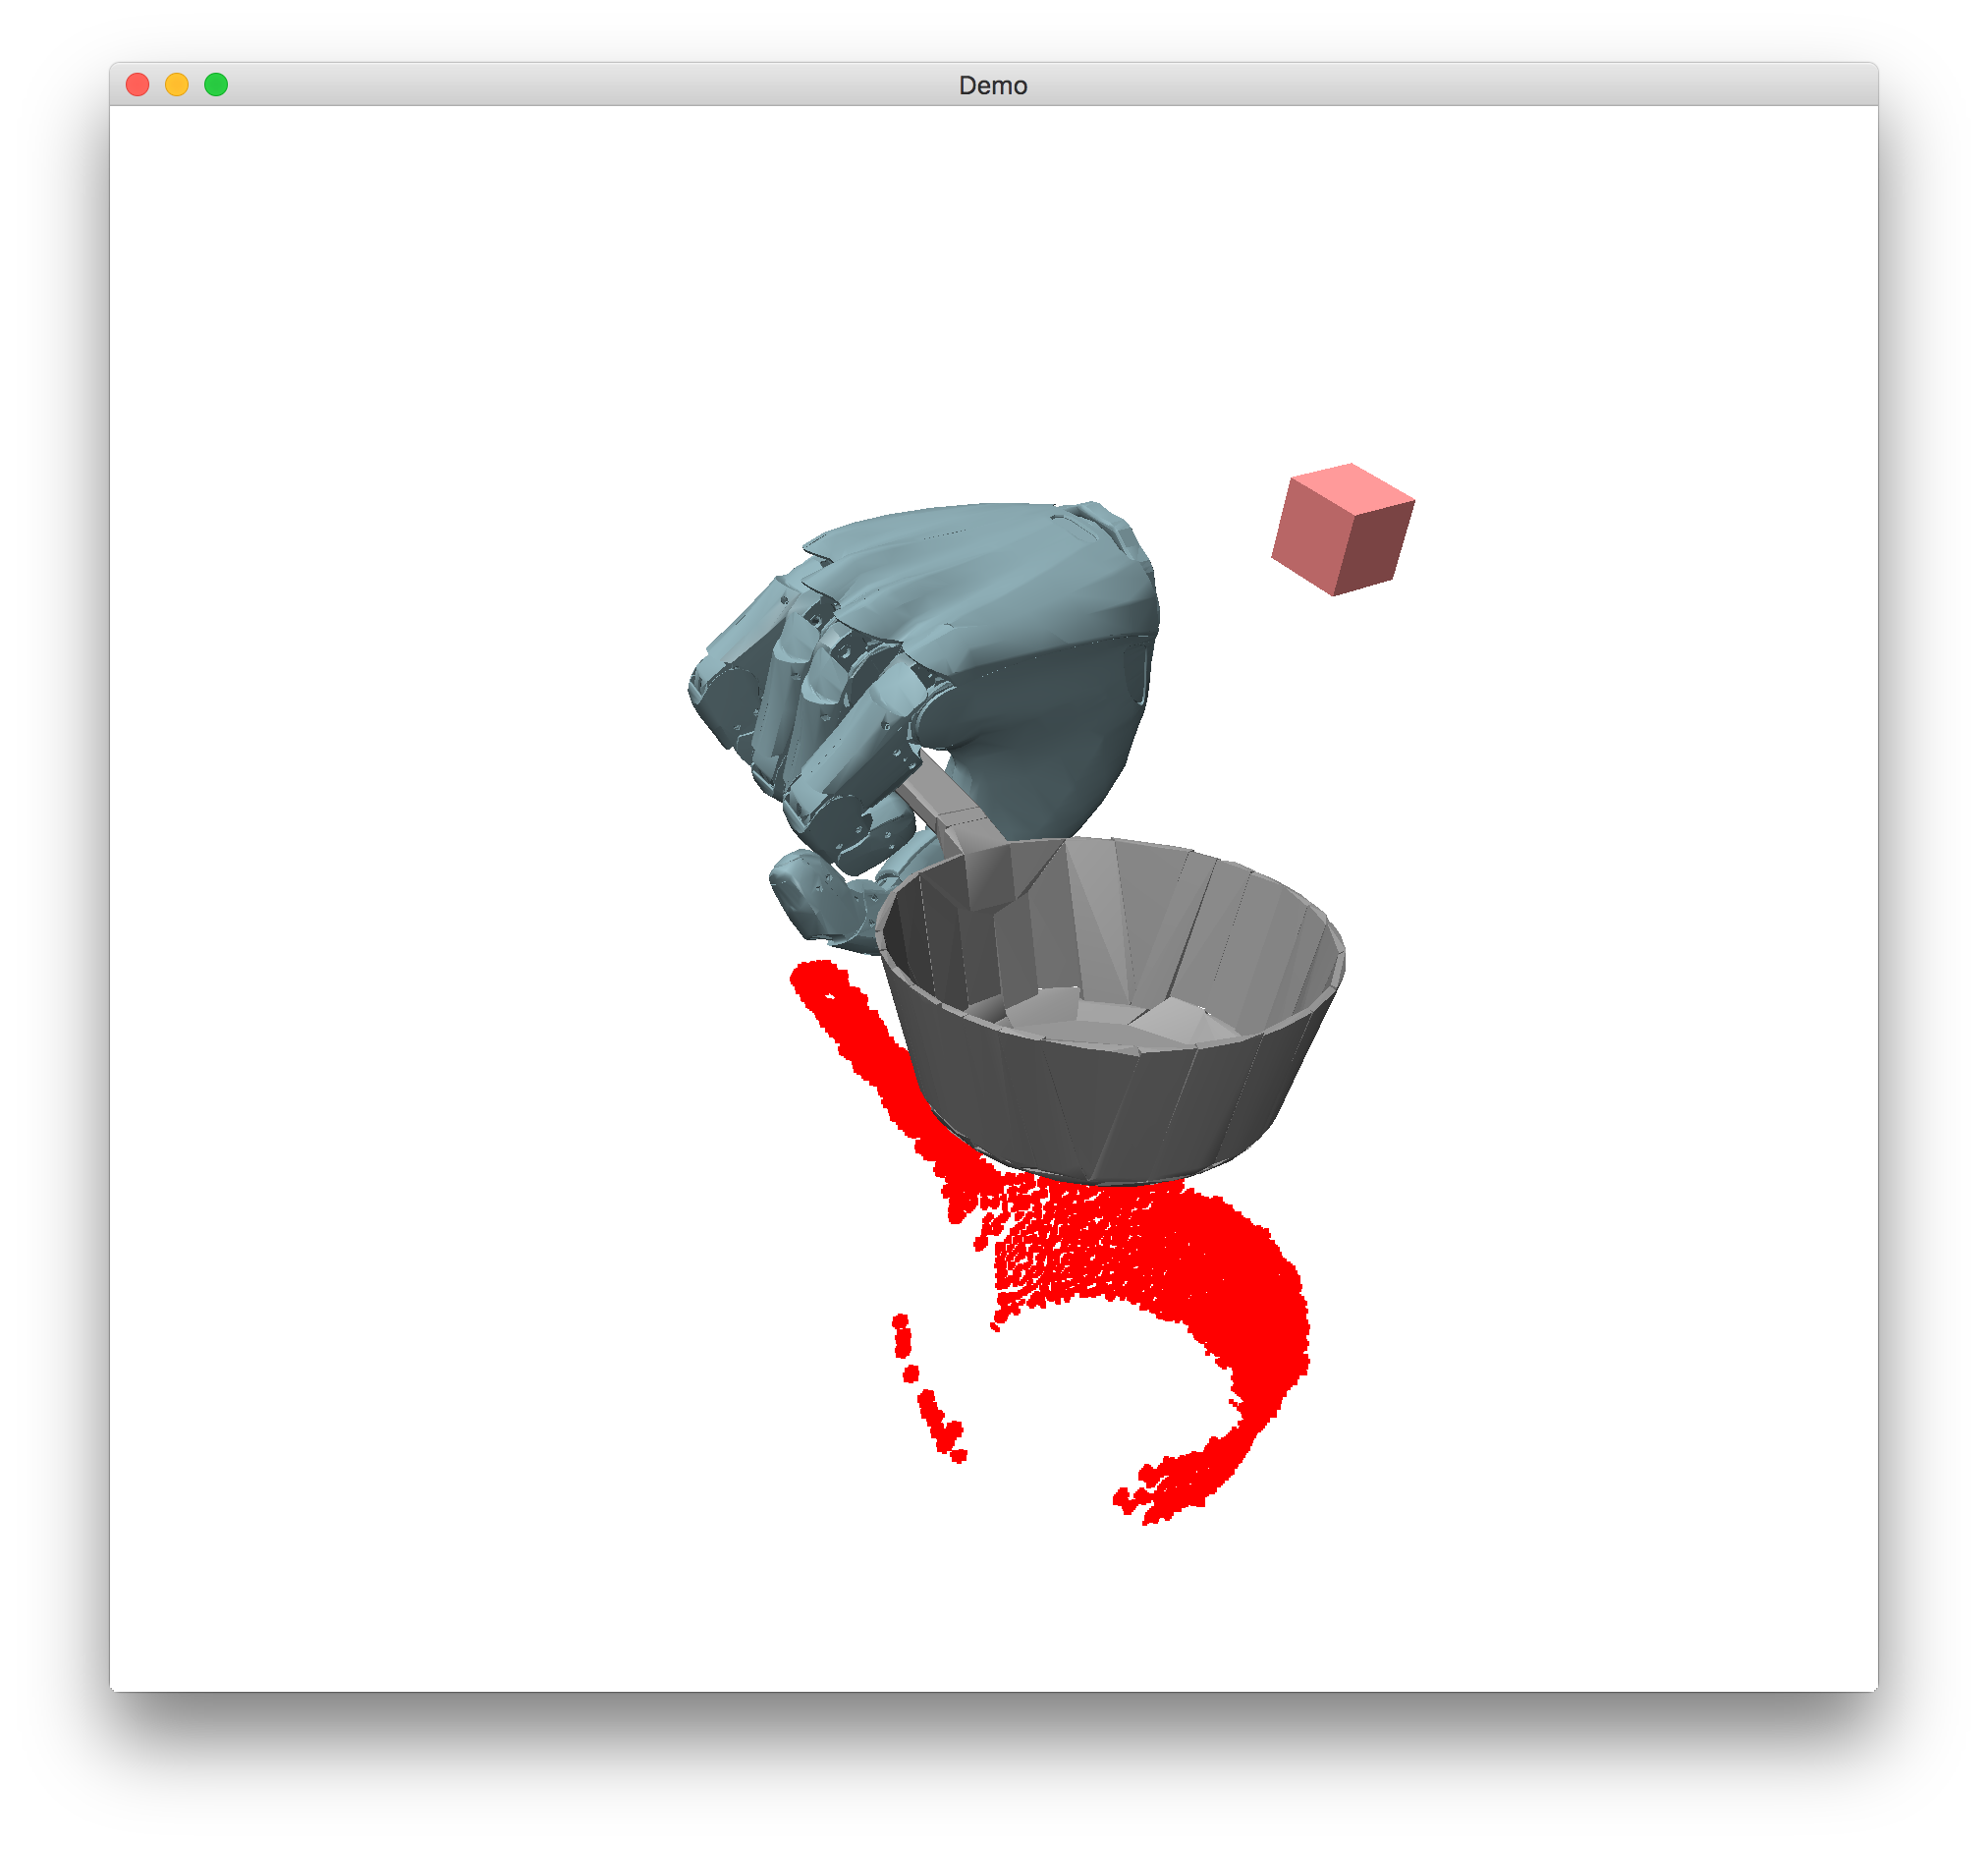
\includegraphics[width=0.24\textwidth]{images/Pan4_LFLW}
%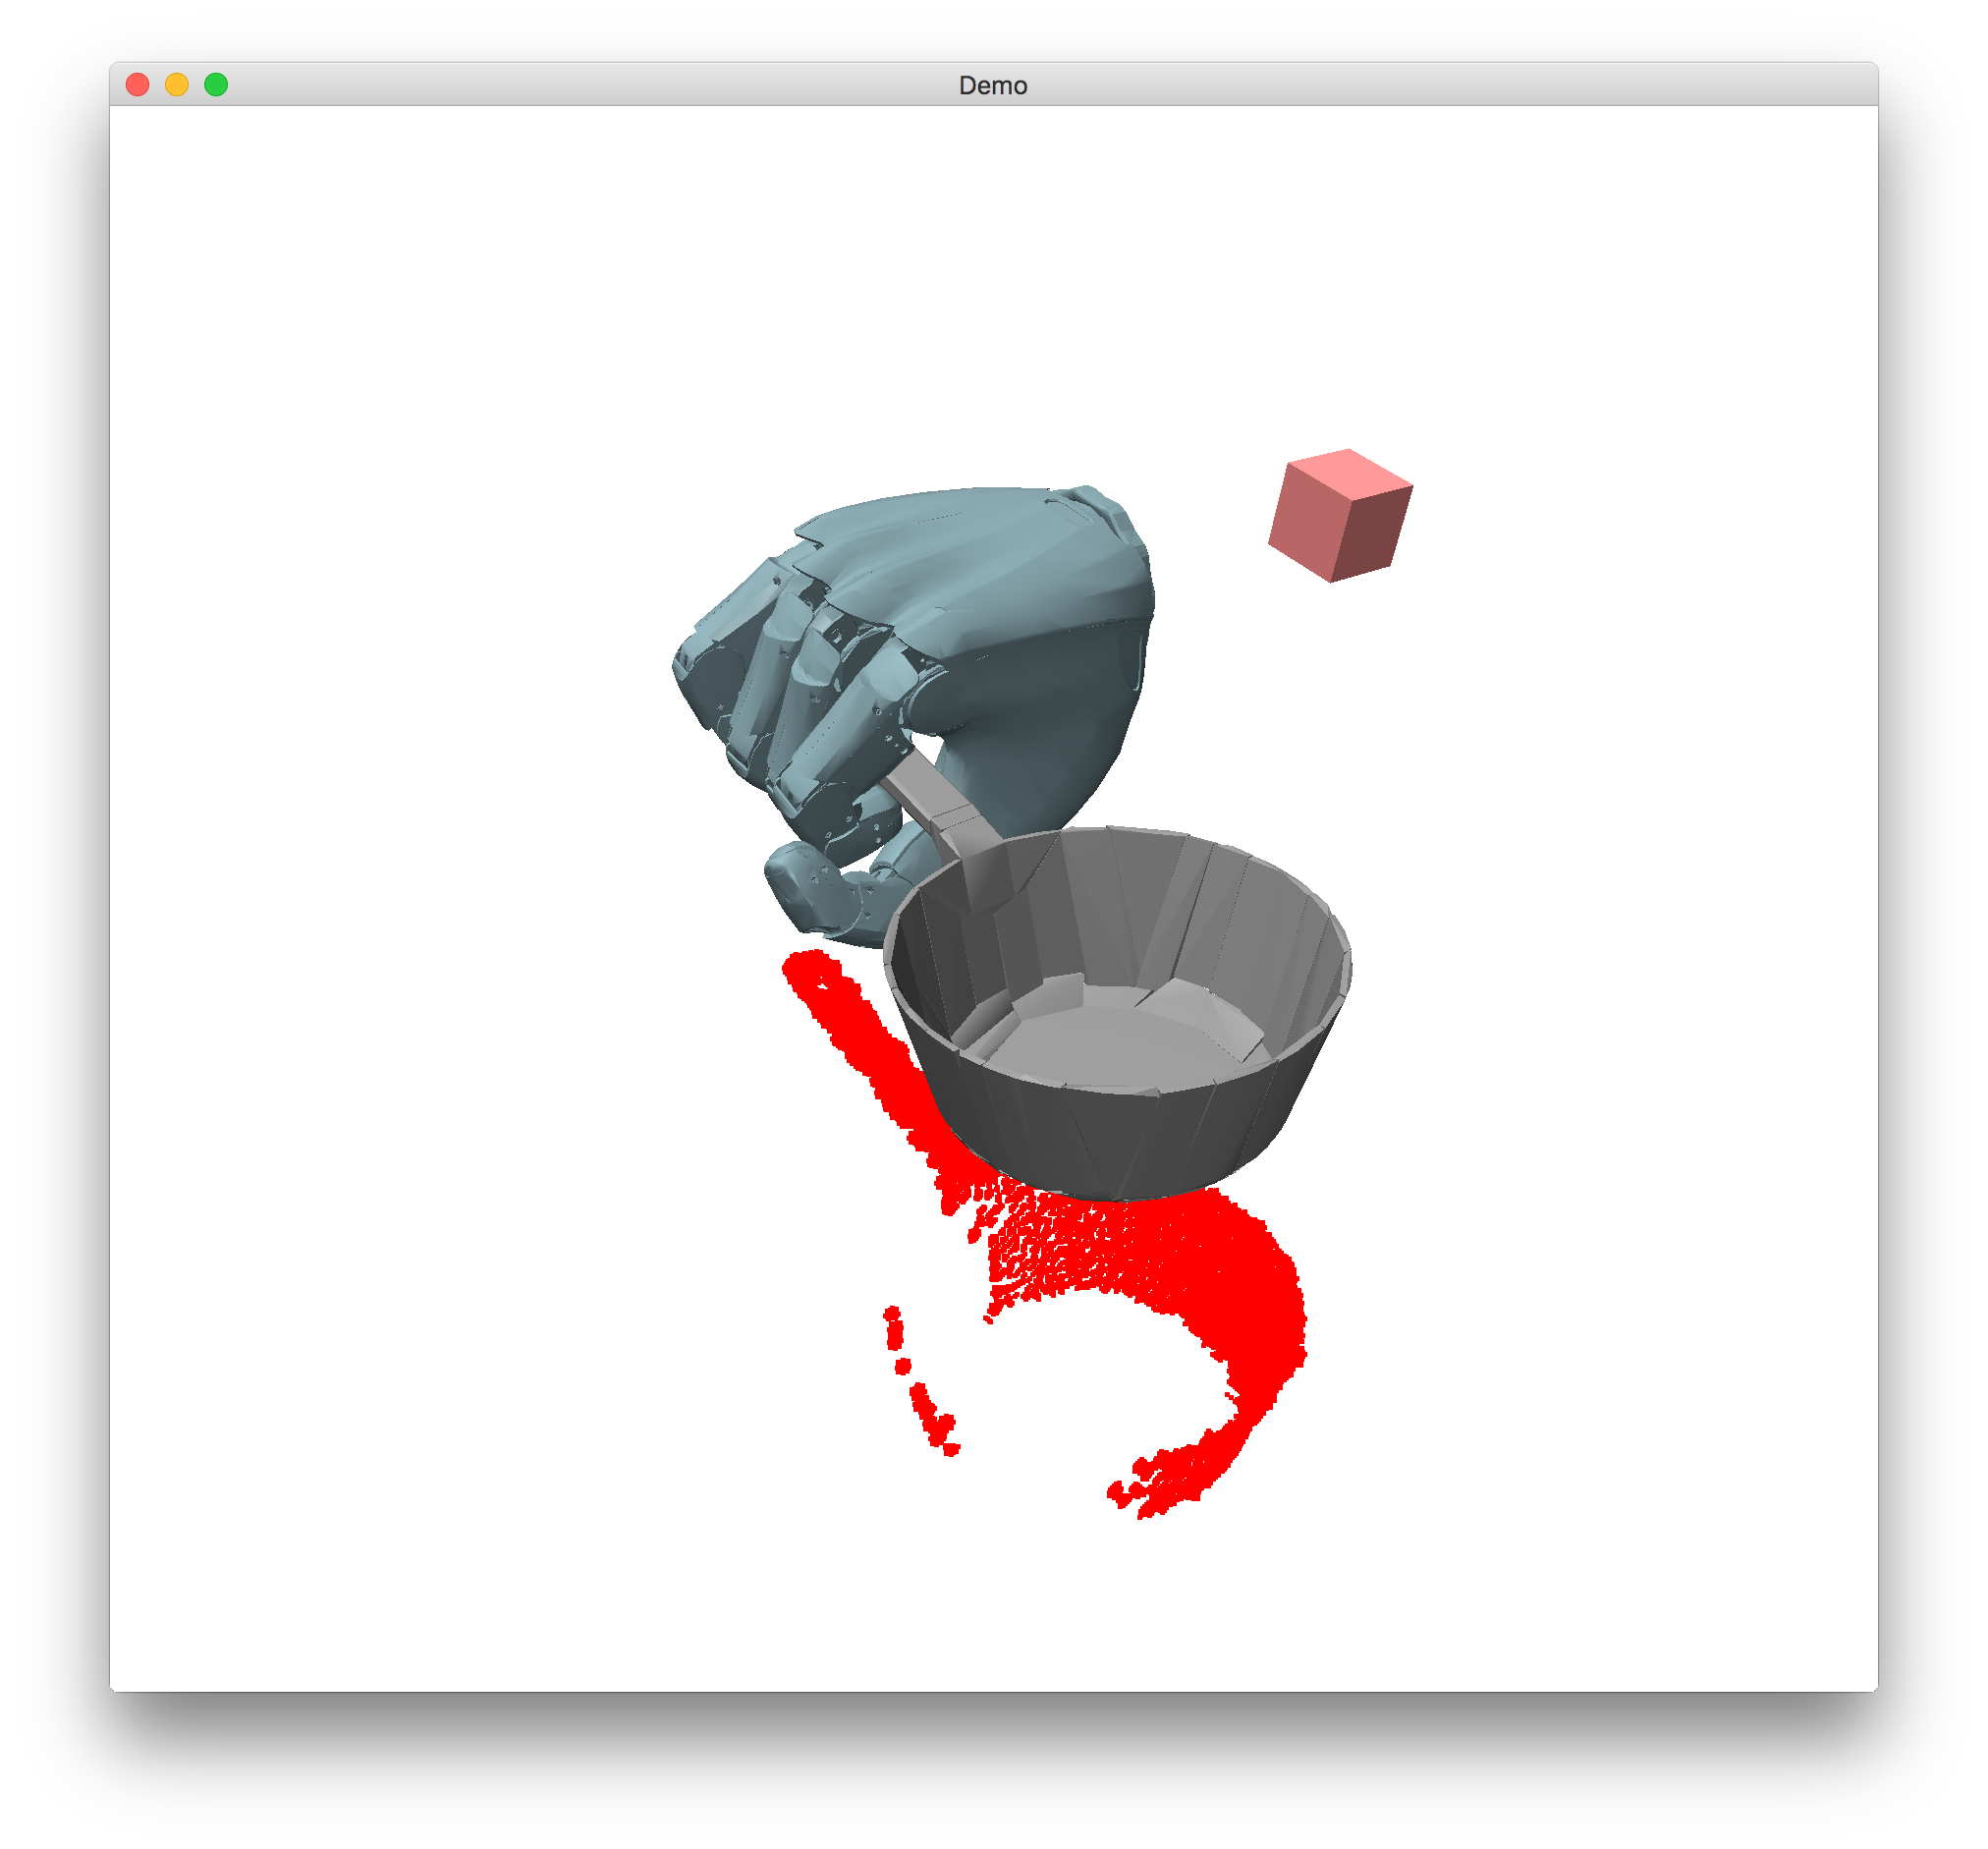
\includegraphics[width=0.24\textwidth]{images/Pan4_HFHW}
%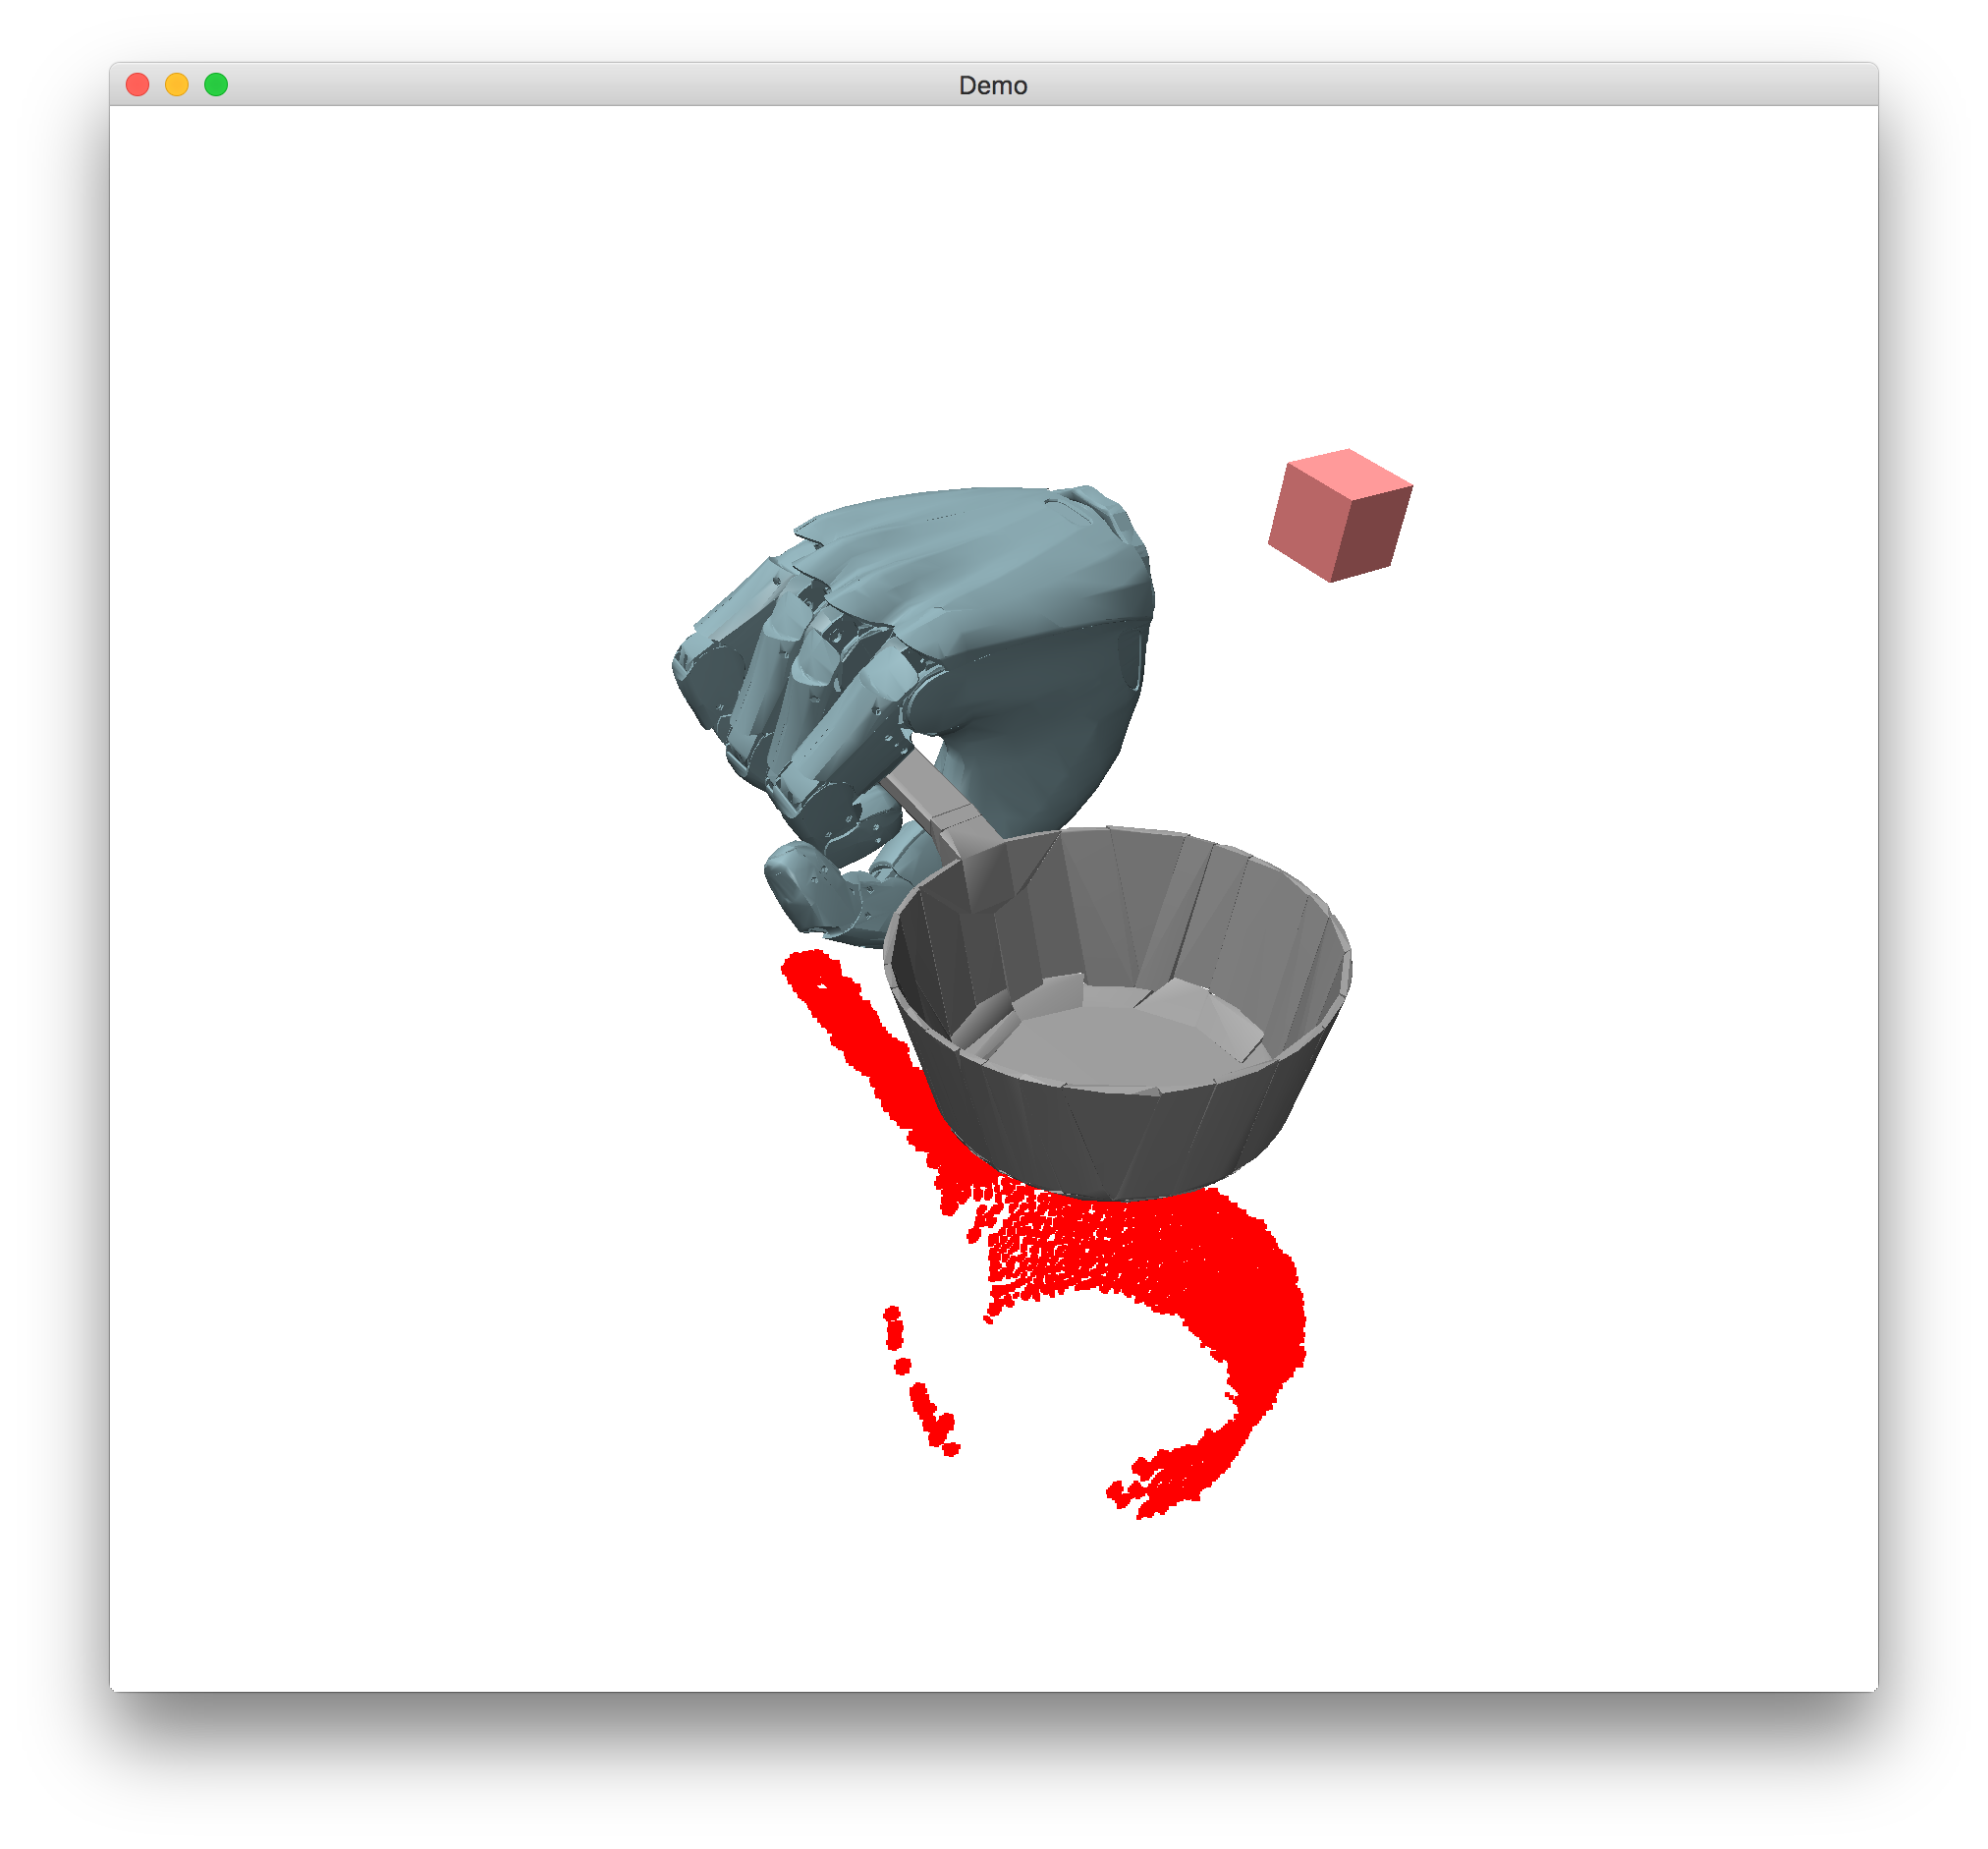
\includegraphics[width=0.24\textwidth]{images/Pan4_LFHW}
\caption{Training a robust evaluation model. (Top row) The same pinch grasp, executed on the same object, with varying friction and mass parameters. (Bottom row) A more robust power grasp, executed on the same object, with the same variation in friction and mass. \label{fig:evaluative-training}}
\end{figure}

\begin{figure}[hb]
  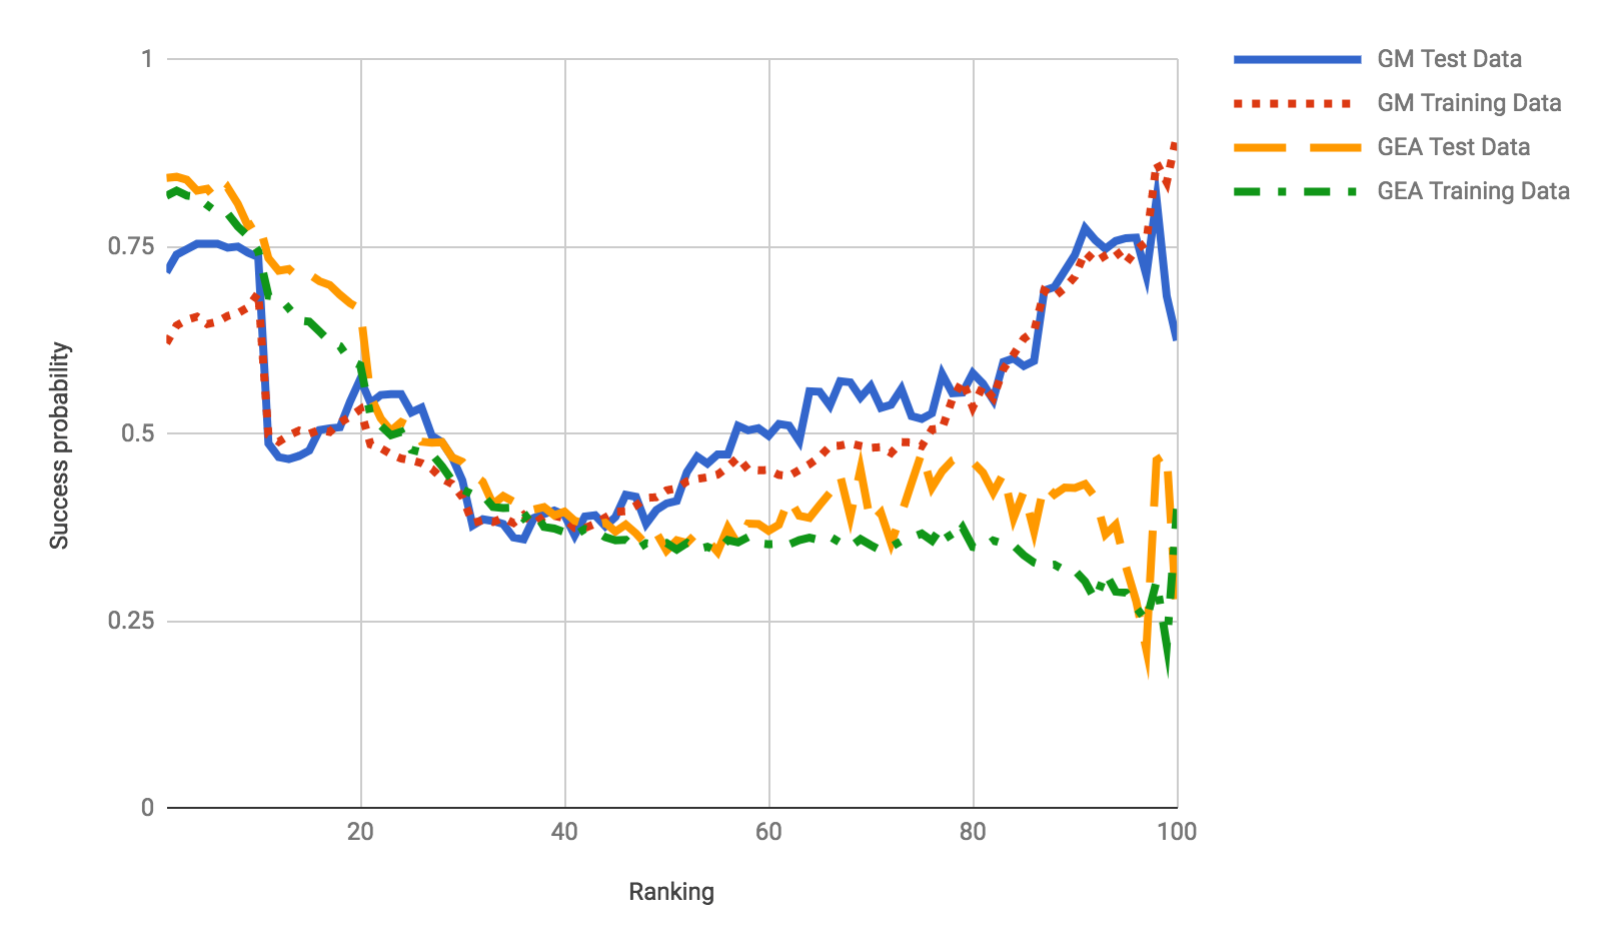
\includegraphics[width=\linewidth]{images/successvsranking.png}
  \caption{Grasp success probability vs. grasp ranking in simulation.}
  \label{fig:successvsranking}
\end{figure}

\begin{table}[h]
\centering
\caption{Precision and recall for grasp success predictions.}
\label{fig:predictions}
\begin{tabular}{|c|c|c|c|c|}
\hline
    & \multicolumn{2}{c|}{\#} & \multicolumn{2}{c|}{\%} \\ \hline
    & PS         & PF         & PS         & PF         \\ \hline
GTS & 33890      & 6353       & 84\%       & 16\%       \\ \hline
GTF & 25631      & 10339     & 71\%       & 29\%       \\ \hline
\end{tabular}
\end{table}
